% !TEX root = ../main.tex

\chapter{Deep learning}
\label{ch:deep_learning}

\section{Introduction to deep learning}
Deep learning is currently one of the trendiest topics in machine learning, a subset of artificial intelligence. Machine learning refers to statistical models that allow computers to perform specific tasks without having been explicitly programmed to solve them. In fact, these models try to find structural patterns within data in order to understand new incoming situations and react in the best possible way accordingly. There exist various techniques in machine learning such as k-NN, SVM, k-means, decision trees, association rules, etc. What mainly differentiates deep learning from these algorithms is the concept of neural networks (see section  \ref{what_is_a_neural_network}), that are combined to form deep neural networks.\\
Neural networks are inspired from the biological neural networks of the brain. These systems try to learn how to solve a problem based on the data they receive as input. Many concrete applications make use of neural networks: autonomous vehicles, smarter translators, personal assistants, art creation, robotics, etc. The presence of deep learning techniques in all mentioned use cases clearly attests that this technology is a real breakthrough. Furthermore, since this field has recently gained interest   (see section \ref{historical_background}), multiple researches are still ongoing, which suggests that many exciting new applications will certainly be discovered.

\subsection{Historical background}
\label{historical_background}
As described in figure \ref{history} from article \cite{14}, the theoretical foundations of deep learning appeared long before the invention of the computers. From the first attempts to understand the human brain until today, a long way has been made to establish the basic components of modern neural networks. One could ask: why did deep learning take off recently if the theory has been around for a long time?\\
First part of the answer is about the computational power. Indeed, deep learning algorithms need a lot of data to work properly and this requires powerful CPU/GPU that either didn't exist or were only available to a minority of people. \\
One other main reason concerns the lack of data. Since deep learning algorithms "learn" from data, if not data is available, no learning is possible. Consequently, the era of Big Data has enhanced the deep learning possibilities.\\
Finally, before the year 2012, the abilities of neural networks had not been publicly proven. This changed with the ImageNet Large Scale Visual Recognition Challenge (a competition where researchers evaluate their algorithms on several visual recognition tasks). In fact, the deep convolutional neural network called "AlexNet" achieved 16\% of classification error rate, whereas the previous best scores were around 25\%. This victory marked the beginning of a new craze for these types of algorithms.



\begin{figure}[!h]
\centering
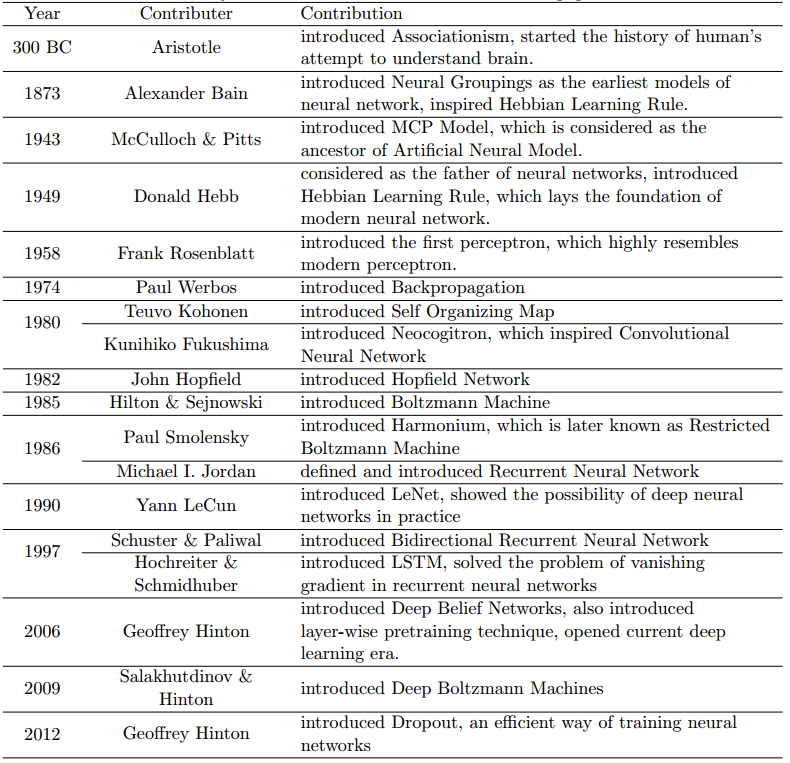
\includegraphics[width=1\textwidth, keepaspectratio=true]{./figures/history.png}
\caption{Milestones }
\label{history}
\end{figure}

 
\subsection{What is a neural network?}
\label{what_is_a_neural_network}

From a descriptive point of view, neural networks can simply be seen as a non linear applications that associate an input to an output with respect to certain parameters. The input can be images, sounds or whatever features that is numerical. The output of a neural network depends on the problem it tries to solve. In computer vision, the most common types of outputs  are classes (for classification problems) and pixel coordinates (for segmentation problems).\\
The figure \ref{neural_network} globally illustrates the concept of a neural network: in a fully connected neural network,  all inputs are given to all neurons of the first layer. Each neuron sums the incoming inputs, passes the result through a non linear function and sends it to all neuron of the next layer along an edge. Each edge between two neurons has a certain weight (a numerical value) that weights the importance of the output of the previous neuron.\\
From a mathematical point of view, a neural network can be defined as a non linear function $f$ that associates to an input $x$ an output $y$ with respect to parameters $\theta$.
\begin{equation}
y = f(x,\theta)
\end{equation}
The parameters $\theta$ are estimated from the training samples.
%\begin{figure}[!h]
%\centering
%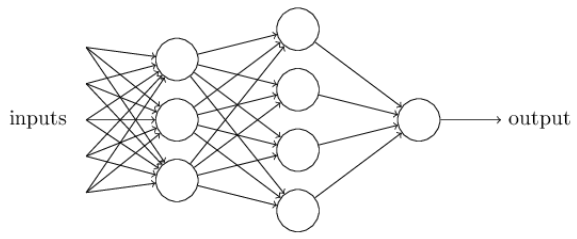
\includegraphics[width=1\textwidth, keepaspectratio=true]{./figures/neural_network.png}
%\caption{Neural Network example}
%\label{neural_network}
%\end{figure}

\begin{figure}[!h]
\centering
	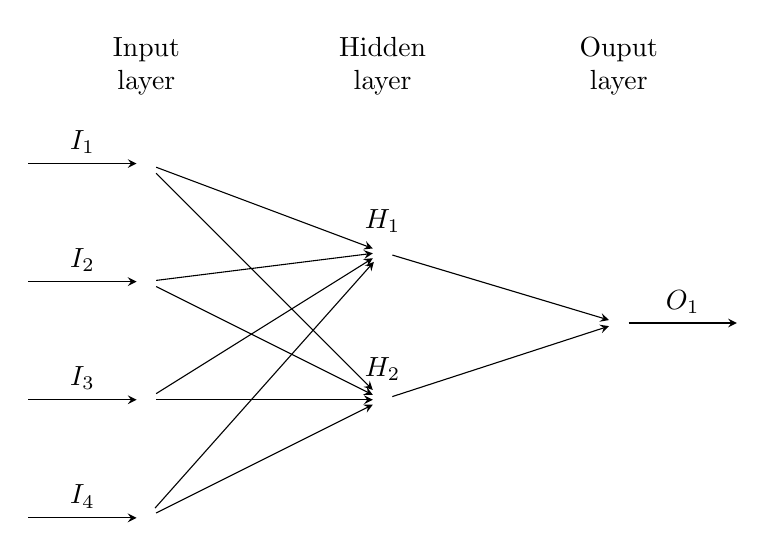
\begin{tikzpicture}[x=1.5cm, y=1.5cm, >=stealth]
	
	\foreach \m/\l [count=\y] in {1,2,3,4}
	  \node [every neuron/.try, neuron \m/.try] (input-\m) at (0,2.5-\y) {};
	
	\foreach \m [count=\y] in {1,2}
	  \node [every neuron/.try, neuron \m/.try ] (hidden-\m) at (2,2-\y*1.25) {};
	
	\foreach \m [count=\y] in {1}
	  \node [every neuron/.try, neuron \m/.try ] (output-\m) at (4,0.15) {};
	
	% input layer
	\foreach \l [count=\i] in {1,2,3,4}
	  \draw [<-] (input-\i) -- ++(-1,0)
	    node [above, midway] {$I_\l$};
	
	% hidden layer
	\foreach \l [count=\i] in {1,2}
	  \node [above] at (hidden-\i.north) {$H_\l$};
	
	% output neurons
	\foreach \l [count=\i] in {1}
	  \draw [->] (output-\i) -- ++(1,0)
	    node [above, midway] {$O_\l$};
	
	% input -> hidden
	\foreach \i in {1,...,4}
	  \foreach \j in {1,...,2}
	    \draw [->] (input-\i) -- (hidden-\j);
	
	% hidden -> output
	\foreach \i in {1,...,2}
	  \foreach \j in {1}
	    \draw [->] (hidden-\i) -- (output-\j);
	
	% labels above layers
	\foreach \l [count=\x from 0] in {Input, Hidden, Ouput}
	  \node [align=center, above] at (\x*2,2) {\l \\ layer};
	
	\end{tikzpicture}
\caption{Neural Network example}
\label{neural_network}
\end{figure}



\section{Neural networks basics}

\subsection{Perceptrons}
\label{perceptron}


\subsection{Multilayer perceptron}


\subsection{Forward propagation}


\subsection{Backpropagation}

\subsubsection{Loss function}

\subsubsection{Weight update}




\section{Training a neural network}

\subsection{Data}
Training set, validation set, test set, supervised learning, unsupervised learning,

\subsection{Weight initialization}

\subsection{Hyperparameters}
lr, batch size, epochs, optimizer, learning rate decay, ...




\section{Deep learning models}
xxx

\subsubsection{Convolutional Neural Networks}


\subsubsection{Recurrent Neural Networks}




\section{Transfer learning}




\section{Deep learning frameworks}